\documentclass[border=6pt]{standalone}
\usepackage[T1]{fontenc}
\usepackage{lmodern}
\usepackage{pgfplots}
\pgfplotsset{compat=1.16}
% Generated by make_result_figure.py from run_github_39307634508/panel/result.json.
\begin{document}
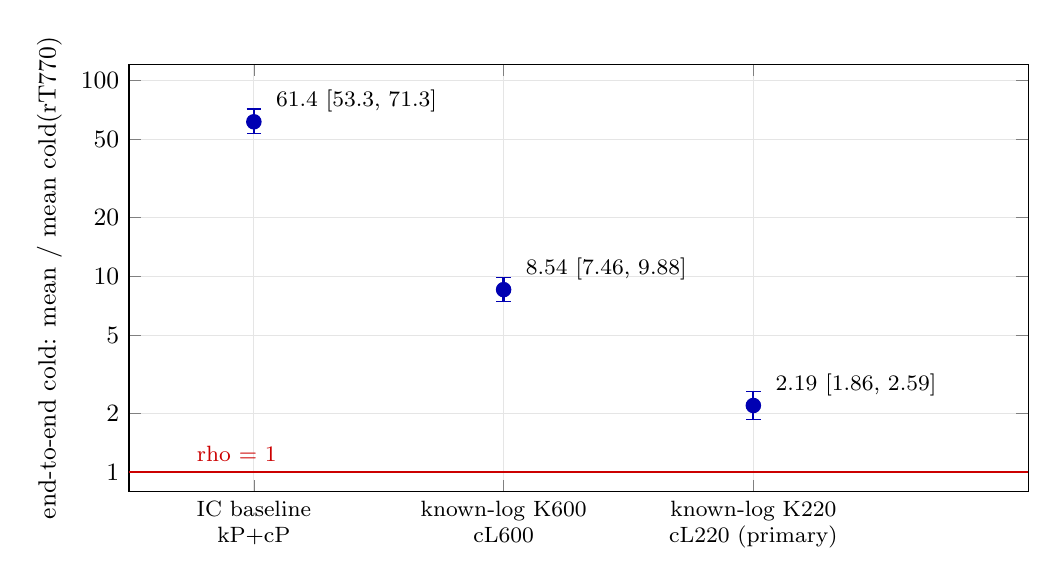
\begin{tikzpicture}
\begin{axis}[width=13cm, height=7cm, ymode=log, ymin=0.8, ymax=120, xmin=-0.5, xmax=3.1,
  ylabel={end-to-end cold: mean / mean cold(rT770)},
  xtick={0,1,2}, xticklabels={{IC baseline\\kP+cP},{known-log K600\\cL600},{known-log K220\\cL220 (primary)}}, x tick label style={font=\footnotesize, align=center},
  grid=major, grid style={gray!20}, font=\small, log ticks with fixed point, ytick={1,2,5,10,20,50,100}]
\addplot[only marks, mark=*, mark size=2.6pt, blue!70!black, error bars/.cd, y dir=both, y explicit,
  error bar style={thick, blue!70!black}] coordinates {(0,61.3504) += (0,9.9274) -= (0,8.0887) (1,8.5446) += (0,1.3355) -= (0,1.0873) (2,2.1919) += (0,0.3974) -= (0,0.3335)};
\draw[red!80!black, thick] (axis cs:-0.5,1) -- (axis cs:3.1,1) node[pos=0.12, above, font=\footnotesize] {rho = 1};
\node[font=\footnotesize, anchor=south west] at (axis cs:0.05,61.35) {61.4 [53.3, 71.3]};
\node[font=\footnotesize, anchor=south west] at (axis cs:1.05,8.54) {8.54 [7.46, 9.88]};
\node[font=\footnotesize, anchor=south west] at (axis cs:2.05,2.19) {2.19 [1.86, 2.59]};
\end{axis}
\end{tikzpicture}
\end{document}
